\documentclass[10pt]{article}
\usepackage[german]{babel}
\usepackage[utf8]{inputenc}
\usepackage{amssymb}
\usepackage{listings}
\usepackage{enumitem}
\usepackage{fancyhdr}
\usepackage{titling}
\usepackage{pgf}
\usepackage{tikz}
\usepackage{array}
\usepackage{ragged2e}

\usetikzlibrary{arrows,automata}
% \usepackage[latin1]{inputenc}

\title{Informatik 3 Übung - Teil 2\vspace{-2ex}}
\author{Daniel Brun, Michael Hadorn\vspace{-2ex}}

\setlength{\droptitle}{-6em}     % Eliminate the default vertical space
\addtolength{\droptitle}{-4pt}   % Only a guess. Use this for adjustment

\newcolumntype{P}[1]{>{\centering\hspace{0pt}}p{#1}}

\pagestyle{fancy}
% clear any old style settings
\fancyhead{}
\fancyfoot{}

\lhead{ZHAW: Informatik 3}
\rhead{Daniel Brun, Michael Hadorn, Inf 3b}
\fancyfoot[LE,RO]{\thepage}

\usepackage{color}

\begin{document}
\maketitle

% Aufgabe 1  	a: OK	b: OK	c: OK	d: 
\section{Aufgabe}
Gegeben sei ein Prozessor mit einer Taktzykluszeit von 1.25 GHz und einem CPI-Wert von 1.45 (der Prozessor verfügt über keine Pipeline). Ein Programm benötigt zur Ausführung 150‘000 Befehle.

\begin{enumerate}[label=\alph*)]
	\item 
	\textit{Wie lang ist die ungefähre Ausführungszeit des	Programms? Lösung: (3 Punkte)}
	
	$ (1 / 1.25 GHz)*(150'000 * 1.45) = 1.74 * 10^{-4} s$
	
	\item
	\textit{Wieso ist der berechnete Wert nur ein Näherungswert? Lösung: (2 Punkte)}\\
	Da der CPI-Wert der Durchschnitt der Zyklen eines Befehles definiert, kann man daraus nicht folgern, dass sich der Zeit-Aufwand der Ausführung genau aus diesem ableiten lässt. Wenn es z.B. mehrere Befehle gibt, die mehrere Zyklen benötigen, so wird die Ausführung länger dauern.
	\item
	\textit{Der Prozessor wird durch einen leistungsfähigeren Prozessor mit 0.4 ns Taktzykluszeit und einem CPI-Wert von 1.8 ersetzt. Wie lang ist nun die Ausführungszeit des Programms? Lösung: (2 Punkte)}
	
	$ (150'000*1.8)*(0.4*10^{-9}) = 0.000108 s = 1.08 * 10^{-4} s$\\
			
	\item
	\textit{Der Prozessor (von c) wird um 10\% übertaktet ("overclocking"). Die erzielte Leistungssteigerung beträgt in der Realität aber nur knapp 5\%. Wieso? Lösung: (2 Punkte)}
	
	%TODO vielleicht ;) Stern hat im Unterricht was erwähnt, in den Folien steht es leider nicht. Der Buss könnte es sein, bin mir aber nicht sicher.
	Die Leistung eines Prozessors wird nicht nur durch die Taktzykluszeit bestimmt (diese wird beim Übertakten erhöht). Neben der Taktzykluszeit spielt auch die umgebende Hardware (Speicher, etc.) eine Rolle. Auch kann es sein, dass je nach Einteilung der Befehlsgruppen die Leistungssteigerung in einem Bereich erzielt wird, welcher nicht alltägliche / seltene Befehle beinhaltet.
	%Weil die Busse nicht mithalten können. Das heisst	der CPU muss öfters auf die Daten warten und kann nichts machen. Die Ausführung dauert darum nicht schneller.
	
\end{enumerate}
\newpage

% Aufgabe 2		a:	OK b: OK
\section{Aufgabe}
Gegeben sei ein einfacher Prozessor ohne Pipelining mit einer Wortbreite von 2 Byte (für Daten und Befehle). 
\begin{enumerate}[label=\alph*)]
	\item 
	\textit{Welchen Wert beinhaltet der Befehlszähler jeweils nach Ausführung der jeweiligen Befehle der folgenden Befehlssequenz (der Initialwert sei 24'048 für den ersten Befehl): Ladebefehl, Ladebefehl, Addition, unbedingter Sprung um -12, Speicherbefehl, unbedingter Sprung um + 8, Addition... ? Lösung: (4 Punkte)}
	
	Initial: 24'048\\
	1. Ladebefehl: 24'049\\
	2. Ladebefehl: 24'050\\
	3. Addition: 24'051\\
	4. Unbedingter Sprung: 24'039 \\
	5. Speicherbefehl: 24'040\\
	6. Unbedingter Sprung: 24'048 \\
	...
	\item
	\textit{Was sehen Sie als Informatiker sofort? Lösung: (2 Punkte)}
	
	Es Handelt sich um eine Endlosschleife / Nicht-Terminierenden-Code.
		
\end{enumerate}

\newpage

% Aufgabe 3		a:	OK	b:	OK
\section{Aufgabe}
Gegeben sei ein Prozessor mit 4-stufiger Pipeline (die vier Stufen, wie in der Vorlesung angegeben) und folgender Ausschnitt einer Programmabfolge: 
..., Load, Sprung, Addition, ODER-Operation, Store, Subtraktion, Sprung, AND-Operation, ...
\begin{enumerate}[label=\alph*)]
	\item 
	\textit{Skizzieren Sie graphisch eine (mögliche) Ausführungsabfolge, unter der Annahme, das beim 1. Sprung zu einer nicht vorhergesehenen Adresse gesprungen wird ("`branch prediction"' war falsch).}
	
	\begin{tabular}{r | c | c | c | c | c | c | c | c | c }
	Schritt & 1 & 2 & 3 & 4 & 5 & 6 & 7 & 8 & 9\\
	\hline
	Load		&	L	&	D	&	O	&	E	\\
	Sprung		&	&	L	&	D	&	O	& 	E 	\\
	Addition	&	&	&	L	&	D	&	O	&	E	\\
	ODER-Operation	&	&	&	&	L	&	D	&	O	&	E	\\
	Store	&	&	&	&	&	L	&	D	&	O	&	E	\\
	Pipeline Flush &	&	&	&	&	&	&	&	&\\
	...		&	&	&	&	&	&	L	&	D	&	O	&	E	\\
	\end{tabular}\\
	L: Befehl laden\\
	D: Befehl decodieren\\
	O: Operantend bereitstellen\\
	E: Operationen ausführen\\
	\item 
	\textit{Beschreiben Sie in Ihren Worten, was ein "`pipeline flush"' bedeutet. Lösung: (2 Punkte) }
	
	Wurde ein Befehl falsch geraten ("Branch prediction" lag falsch), müssen die bereits "voraus" bearbeiteten Befehle wieder entfernt und an der korrekten Stelle weitergefahren werden.
	
\end{enumerate}
\newpage

% Aufgabe 4		a: OK
\section{Aufgabe}
Eine effektive Möglichkeit der Leistungssteigerung bei Prozessoren ist Pipelining.
\begin{enumerate}[label=\alph*)]
	\item 
	\textit{Begründen 	Sie, warum eine n-stufige Pipeline nicht automatisch zu einer n-fachen Leistungssteigerung führt, selbst wenn es gelingt, die Zykluszeit auf 1/n zu reduzieren ("`perfekte Gleichverteilung"' der Stufen - in der Praxis eigentlich nicht realisierbar). Lösung:(4 Punkte)}
	
	Beim Pipelining wird nach dem Laden des Befehls bereits der nächste Geladen, dies setzt voraus, dass der nachfolgende Befehl mit einer hohen Genauigkeit vorausgesagt werden kann ("`Branch Prediction"'). Durch die spezielle Architektur, die für das Pipelining notwendig ist, erhöht sich die Komplexität innerhalb des Prozessores um ein vielfaches. Durch die zusätzlich notwendigen Mechanismen zur Kontrolle, Abschirmung, etc. wird auch Leistung benötigt, was der Grund dafür ist, dass keine n-fache Leistungssteigerung erzielt werden kann. Auch kann es vorkommen, dass wenn die Branch-Prediction oft falsch ist, keine grosse Leistungssteigerung erzielt werden kann.
\end{enumerate}
\newpage

% Aufgabe 5		a:	OK	b:	OK	c:	OK	d:	
\section{Aufgabe}
Gegeben sei ein Prozessor ohne Pipeline mit der "`bekannten"' Befehlsabarbeitung (siehe Vorlesung) und einer Zykluszeit von 20MHz. Ein Analyse hat ergeben, dass die einzelnen Teilschritte sehr unterschiedliche Zeit erfordern:\\
z. B. "`Befehl laden"' $\leq$ 10ns, "`Register lesen"' $\leq$ 3ns, "`Rechenoperation durchführen"' $\leq$ 5ns, "`Speicherzugriff"' $\leq$ 20ns und "`Register schreiben"' $\leq$ 5ns, ... \\
Sie implementieren denselben Prozessor mit einer 5-stufigen Pipeline (die bisherigen Teilschritte erfordern gleich viel Zeit). 
\begin{enumerate}[label=\alph*)]
	\item 
	\textit{Wie gross ist die Zykluszeit des neuen Prozessors? Lösung: (3 Punkte) } 
	
	Effektive Zeit der Ausführung eines Befehls:\\
	1s/180000000MHz = 5.555555556e-09s = 5.555556 ns pro Befehl\\
	t = (5 + 5 - 1) * 5.555556 ns = 50.0004 ns\\
	Die neue Zykluszeit beträgt also: 50 ns
	
	% t = (5 + 5 - 1) * 20MHz = 180 MHz \\
	% Die neue Zykluszeit beträgt	180MHz.\\

	\item 
	\textit{Um wie viel schneller wird nun ein Befehl maximal ausgeführt? Lösung: (3 Punkte)} \\
	Der einzelne Befehl wird immer noch gleich schnell ausgeführt. (Idealfall)	
	\item 
	\textit{Um wie viel schneller wird ein Programm maximal ausgeführt? Lösung: (2 Punkte) }
	
	Ein Programm wird nun maximal 5 x so schnell wie vorher ausgeführt. (Idealfall)
	\item 
	\textit{Wie	könnte eine "`bessere"' Pipeline-Struktur entwickelt werden? Lösung: (2 Punkte)  } 
	
	% Sollte der Prozess nicht in mehrere kleinere Stufen aufgeteilt werden (also nicht in weniger Stufen). So können mehrere kurze Befehle gleichzeitig ausgeführt werden. -
	% Könnte auch sein, aber ist das möglich? Befehlszähler auslesen /decodieren, etc. ist ja praktisch schon der "kleinste Schritt" Damit keine Wartezeit entsteht müssten alle Stufen gleich lang sein.
	Es könnten weniger Stufen verwendet werden (geringere Komplexität), Optimierung der Befehlssätze (Format, Datenorganisation, ...). Es müssen alle Komponenten aufeinander abgestimmt sein (Gruppierung der Befehle, etc.).	
\end{enumerate}

\newpage

% Aufgabe 6		a:
\section{Aufgabe}
Eine effektive Möglichkeit der Leistungssteigerung bei Prozessoren ist Pipelining.
\begin{enumerate}[label=\alph*)]
	\item 
	\textit{Recherchieren Sie die Pipelinestruktur und Kenndaten von zwei aktuellen Mikroprozessoren. Bitte Kenndaten angeben und Struktur skizzieren, inkl. Quellenangabe. Lösung: (6 Punkte) }
	
	\textbf{AMD FX Eight-Core-Prozessor Black Edition}\\
	\begin{tabular}{ l l l l l l l }
		Modellnummer & FX 9590\\
		Frequenz & 4.7/5.0 GHz\\
		Gesamter L2-Cache & 8MB\\
		L3-Cache & 8MB\\
		Bauform & Socket AM3+\\
		Leistungsaufnahme & 220W\\
		Fertigungs-Technologie & 32nm SOI\\
		Mikroarchitektur & Bulldozer \\
		Befehlssatz & x86/AMD64 \\
	\end{tabular}
	
	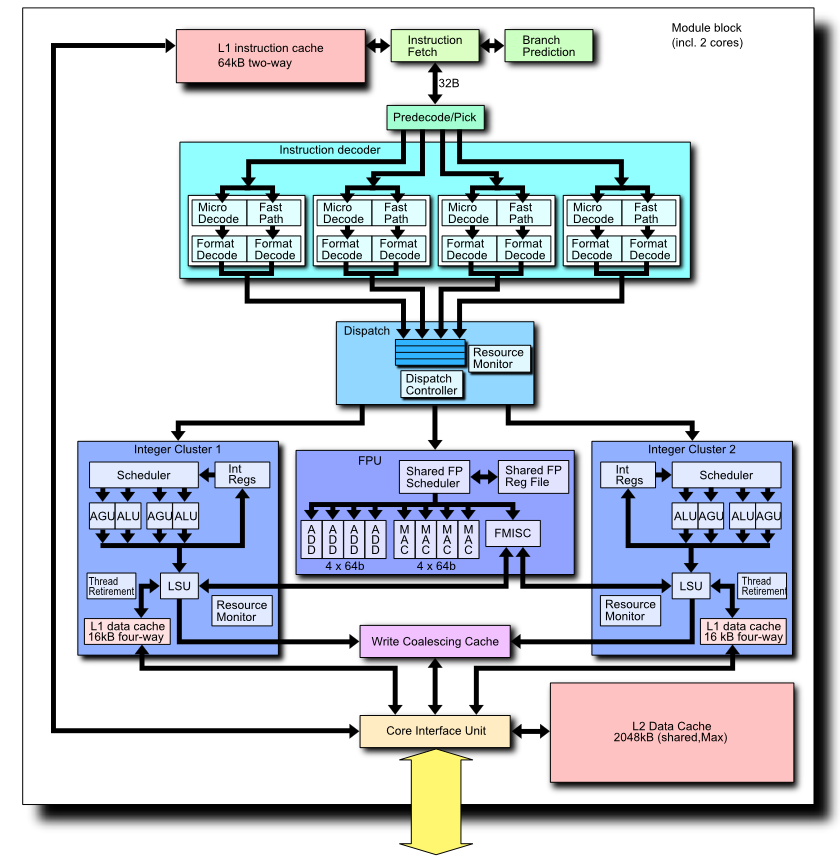
\includegraphics[width=0.85\textwidth]{images/AMD_Bulldozer.png}
	
%	\begin{figure}[!Hhtp]
%	  \centering
%	  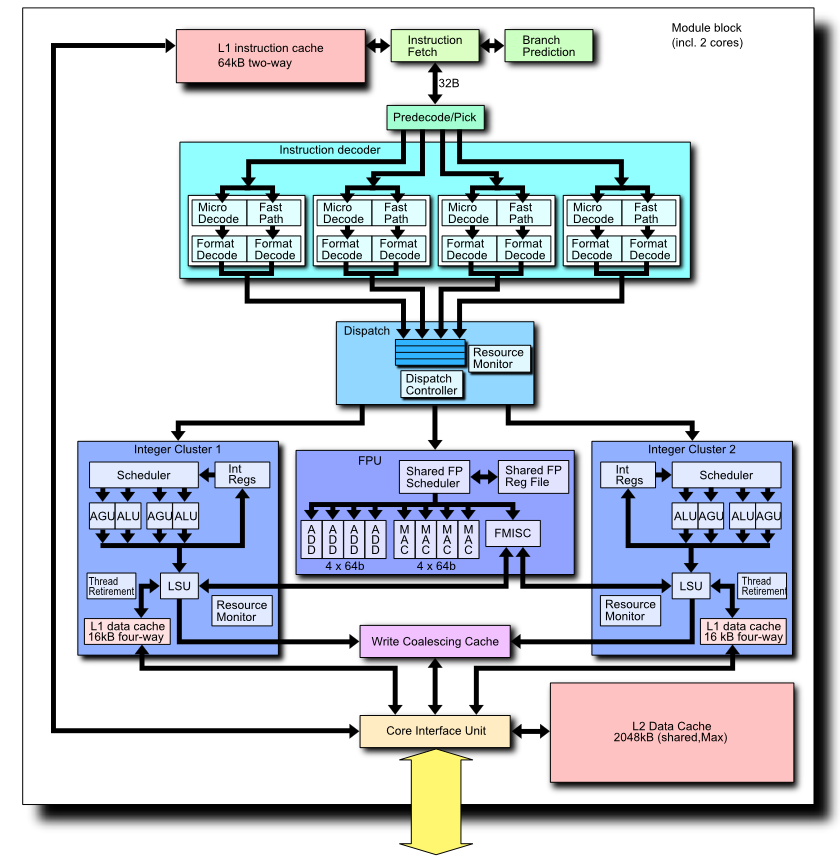
\includegraphics[width=\textwidth]{images/AMD_Bulldozer.png}
%	  \caption[AMD Bulldozer]{Blockdiagramm eines Bulldozer-Moduls}
%	\end{figure}
	
	
	http://www.amd.com/de/products/desktop/processors/amdfx/Pages/amdfx.aspx\\
	http://de.wikipedia.org/wiki/AMD\_Bulldozer\\
	\\
	
	\textbf{Intel Core i7 Sandy-Bridge}\\
	\begin{tabular}{ l l l l l l l }
			Modellnummer & Intel Core i7-4960HQ\\
			Frequenz & 2.6 GHz\\
			Gesamter L2-Cache & 1024 KB\\
			L3-Cache & 6MB\\
			Bauform & LGA 2011\\ 
			Leistungsaufnahme & 47W\\
			% Fertigungs-Technologie & ?? \\
			Mikroarchitektur & Sandy Bridge (E)\\
			Befehlssatz & x86 \\
			Anzahl Kerne/ Anzahl Threads & 4 / 8\\
			Speichertypen & DDR3L-1333,1600\\
			Grafik & Intel® Iris™ Pro graphics 5200\\
		\end{tabular}
	
	% Skizze der Struktur
	% Was meinsch zu dene? http://www.elektroniknet.de/uploads/media_uploads/images/1298475607-39-blockdiagramm-sandybridge.jpg
	%http://pics.computerbase.de/3/2/2/9/8/6.png
	
	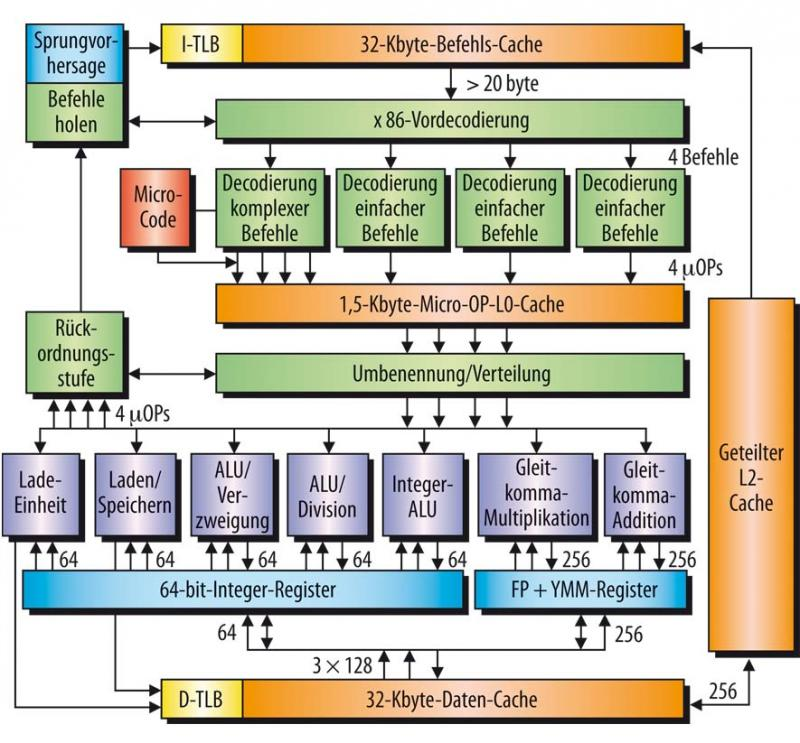
\includegraphics[width=0.85\textwidth]{images/sandybridge.jpg}\\
	Bild: http://www.elektroniknet.de/uploads/media\_uploads/images/1298475607-39-blockdiagramm-sandybridge.jpg\\
	
	http://www.intel.de/content/www/de/de/processors/core/core-i7-processor.html\\
	http://en.wikipedia.org/wiki/Sandy\_Bridge-E\\
\end{enumerate}

\end{document}